\chapter{Research Phase}
\section{Current Modeling Environments}

\subsection{Simile (Simile Visual Modelling Environment)}
Simile is a visual modelling environment, developed originally for the dynamic modelling of ecological and environmental systems, which supports a wide range of ways of representing space. Therefore, it addresses both of the above issues in a single environment.

\emph{Visual modeling environment}
\begin{itemize}
	\item Build model without learning programming
	\item Display concept \& relationship using diagram, for example (stocks, flows and influences)
	\item GUI for simulation control \& specifying inputs
	\item Visualize \& compare the model behaviors in  graphs \& tables
\end{itemize}

\emph{What can we use it for?}
\begin{itemize}
	\item Rate expressions for biological, chemical, or physical processes (differential equations), for example: Mass balance or accounting, Growth dynamics, Respiration
	\item Scenario analysis, for example: Effect of flow velocity on gas exchange between  river-atmosphere
\end{itemize}

\emph{Technical implementation:}\\
\emph{Architecture}\\
The following diagram \ref{fig:Simile Architecture} shows the main components of Simile, and how they relate to each
other.

\begin{figure}[htbp]
\centering
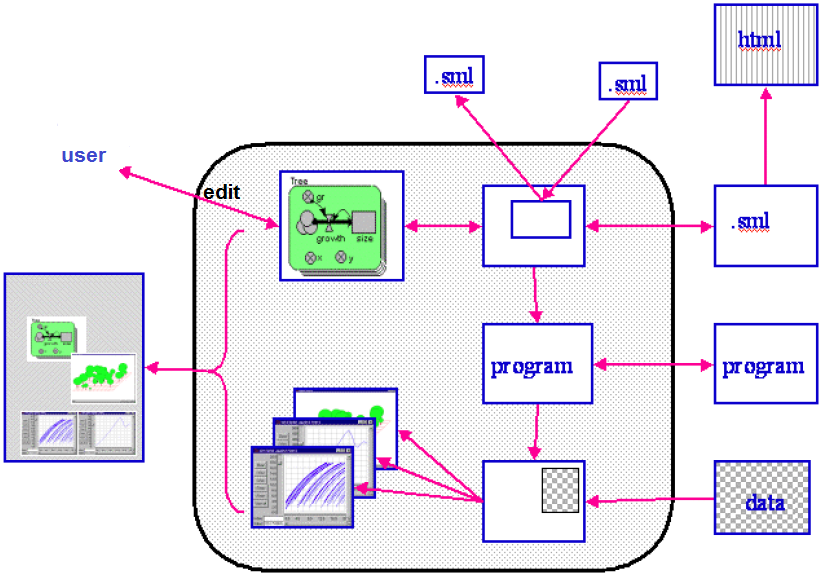
\includegraphics[width=0.6\textwidth]{pics/simile/Simile_architecture.png}
\caption{Simile Architecture}
\label{fig:Simile Architecture}	
\end{figure}

In the middle-left, the user interacts with Simile through a graphical user interface (GUI) to edit the model diagram and equations. In the process, Simile builds up an internal representation of the model, which may contain submodels. The model or a submodel 
(submodel will be explained later) can be saved to file (.sml extension) (arrows going to the top and to the right). Also, a model or a submodel can be loaded from file (arrows coming in from top and right).\\
To run a model, the internal representation is used to generate a program in tcl (Tool command language) or C. (In fact, not shown here is that in C Simile first generates the source code, then compiles it as a DLL (Data Definition Language)). This program can also be saved to file, it is possible to run a previously-built model as a stand-alone executable without having access to the Simile environment. The program may then need to be combined with external data sets, containing parameter and tabulated values. After run, Simile calls on various display tools to show the results of the simulation. The displayed results of the simulation may then be exported, along with the model diagram, to produce a postscript file that can be used to produce a handout or poster about the modelling exercise.\\
At the top-right of the diagram, you will notice that the saved model can be used to generate an html description of the model. This is handled by a program (written in Prolog) that is totally independent of Simile itself. The html generator is the first of many such tools, and ultimately we envisage that many groups around the world will be writing their own for processing Simile models in new and useful ways.

\emph{Properties of the modeling:}\\
Simile has a number of features
	\subsubsection{Visual modelling:}
Simile supports a two-phase approach to model construction. The first involves the drawing of diagrams that show the main features of the model and the second involves fleshing-out the model-diagram elements with quantitative information on the relevant values and equations.
	\subsubsection{System Dynamics:}
Simile allows models to be formulated in System Dynamics terms, as compartments (stocks, levels) whose values are governed by flows in and out. This can be considered as a visual language for representing differential-equation models, with a compartment representing a state variable, and the rate-of-change being the net sum of inflows minus outflows.
	\subsubsection{Disaggregation:}
Simile allows the modeller to express many forms of disaggregation: e.g. age/size/sex/species classes. This is achieved by defining how one class behaves, then specifying that there are many such classes.
	\subsubsection{Object-based modelling:}
Simile allows a population of objects to be modelled. As with disaggregation, model designers state how one member behaves, then specify that there are many such members. In this case, the designer can add in symbols denoting the rules for creating new members of the population, and for killing off existing members. Individual members of the population can interact with others.
	\subsubsection{Spatial modelling:}
It follows that spatial modelling in the system is simply a special form of disaggregation. One spatial unit (grid square, hexagon, polygon, etc.) is modelled, then many such units are specified. Each can be given spatial attributes, such as area or location, and the proximity of one unit to another can be represented.
	\subsubsection{Modular modelling:}
Simile allows any model to be inserted as a submodel into another. Having done this, the modeller can then manually make the links between variables in the two components (in the case where the submodel was not designed to plug into the main model); or links can be made automatically, giving a (plug-and-play) capability. Conversely, any submodel can be extracted and run as a stand-alone model, greatly facilitating testing of the submodels of a complex model.
	\subsubsection{Efficient computation:}
Models can be run as compiled programs. In many cases, these will run as fast as a hand-coded program, enabling Simile to cope with complex models (100s equations; 1000s object instances). While larger or institutional spatial databases are likely to contain millions of object instances, the complexity of modelling, rather than the efficiency of computation, means that dynamic spatial modelling tasks are often more modest in size.
	\subsubsection{Customisable output displays and input tools:}
Simile users can design and implement their own input/output procedures independently. In particular, they can develop displays for model output that are specific to disciplinary norms or other requirements. Once developed, these can be shared with others in the relevant research community.
	\subsubsection{Declarative representation of model structure:}
A Simile model is saved in an open format as a text file (in Prolog syntax). This means that others can develop tools for processing Simile models in novel ways. For example, one group may develop a new way of reporting on model structure, while another may wish to undertake automatic comparison of the structure of two similar models. It also opens the way for the efficient transmission of models across the Internet (as XML files), and for the sharing of models between different modelling environments.\\
	
In fact, Simile has no particular spatial representations built into it, rather these are specified by the user in Simile's modelling language and this means that modellers have considerable flexibility in just how space is represented. They are not restricted to some pre-defined spatial framework. One model can include both field and object views, polygonal, rectangular and hexagonal areal units, 3D units (e.g. cubes), and point and linear features, all referenced to a common co-ordinate system. Together with appropriate visualisation tools, this flexibility enables a very wide range of dynamic spatial models to be developed.\\
	
\emph{The Simile visual modelling environment allow to:}
\begin{itemize}
	\item draw the elements of model, and the relationships between them
	\item add influences between related variables
	\item using simple mouse actions, to re-arrange the elements, annotate the diagram or add graphics
\end{itemize}	
	
\emph{System Dynamics symbols}

\begin{figure}[htbp]
\centering
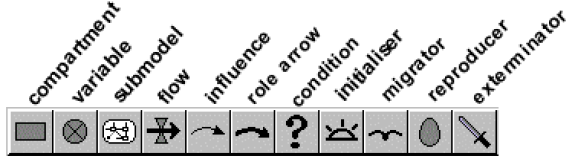
\includegraphics[width=0.6\textwidth]{pics/simile/Simile_symbols.png}
\caption{Simile Symbols}
\label{fig:Simile Symbols}	
\end{figure}

\begin{itemize}
	\item \emph{compartment :}\\
The compartment symbol is used to represent a quantitative state variable
	\item \emph{Variable :}\\
A variable is used to hold one or more values. The value or values come from a mathematical expression
	\item \emph{Submodel :}\\
In Simile, a submodel is a round-cornered box that encloses a number of model-design symbols, including possibly other submodels
	\item \emph{Flow arrow:}\\
The flow arrow is used to specify a term contributing to the rate of change of a compartment
	\item \emph{Influence arrow :}\\
To say that (A influences B) means that A is used to calculate a value for B
	\item \emph{Role arrow :}\\
Role arrows are usually used in pairs, with each arrow going from a submodel to a submodel. The combination of submodels and role arrows is used to denote an association between the objects represented by the submodels at the start of each role arrow
	\item \emph{Condition :}\\
A condition element is placed inside a submodel to indicate that the existence of the submodel depends on some condition
	\item \emph{Initial-number :}\\
The initial-number element is used to specify the initial number of members in a population of objects
	\item \emph{Migrator :}\\
The migrator element is used to specify the rate at which new members of a population are created
	\item \emph{Reproducer :}\\
The reproducer element is used to specify the rate at which each member of a population creates new members
\item \emph{Exterminator :}\\
The mortality element is used to specify the rule for killing off a member of a population of objects
\end{itemize}	

In common with other visual modelling environments, Simile models are built in two phases. First, the modeller produces a diagram. Then, the modeller quantifies the model by entering numeric values and equations for the various components of the model.\\
The diagramming icons are chosen from the Toolbar of simile, the compartment, flow, variable and influence, are concerned with conventional System Dynamics modelling, shown in Figure \ref{fig:The model diagram}.

\begin{figure}[htbp]
\centering
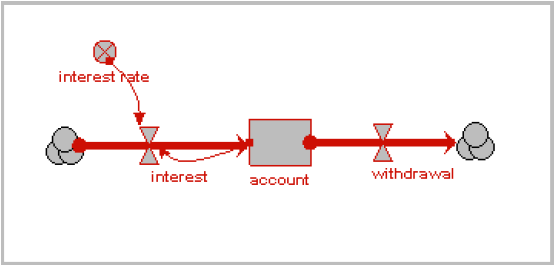
\includegraphics[width=0.6\textwidth]{pics/simile/account_example.png}
\caption{the model diagram}
\label{fig:The model diagram}	
\end{figure}

System Dynamics (SD) is a common dynamic modelling paradigm within the ecological and environmental research communities. A SD model consists of compartments (stocks, levels, storages) connected by flows, with subsidiary variables for representing parameters and intermediate variables, and influence arrows to show which compartments and variables are used in the calculation of flows and other variables. Essentially, SD is a cosmetic language for defining differential- or difference-equation models: differential equations if the equations are taken to define continuous change; difference equations if the time step is taken to be unity.\\

\emph{Concern following problems of simile}
\begin{itemize}
	\item effort and skill needed to program the models
	\item the lack of transparency in models implemented as programs
	\item and the lack of reuseability of models and submodels
\end{itemize}


	
\subsection{esmf (Earth System Modeling Framework)}
The ESMF is an abbreviation for Earth System Modeling Framework. ESMF is an Open Source project used at a broad spectrum of research and operational centers, including the National Weather Service, United States Army Air Forces, the Navy, NASA, and universities.\\
ESMF is used for building and coupling weather, climate, and other Earth science models. This is high-performance software that facilitates interoperability, performance portability, and reuse in numerical weather prediction, climate, data assimilation, and other Earth and space science applications. These applications are computationally intensive and usually run on supercomputers. ESMF includes re-gridding tools for composing complex, coupled modeling systems, and data structures and utilities for developing individual models. The architecture for that is defined by the ESMF team.

\emph{Technical implementation:}\\
ESMF provides a complete set of Fortran interfaces and some C and C++ interfaces.\\
ESMF is based on principles of component-based software engineering. It is a reuse-based approach to defining, implementing and composing loosely coupled independent components into systems. In ESMF, components can create and drive other components so that an ocean biogeochemistry component can be part of a larger ocean component.

\emph{Architecture}\\
The view of the framework consists of two layers, an infrastructure of utilities and data structures for creating model components, and a superstructure for coupling them. User code is placed between these two layers, to make calls to the infrastructure libraries and be scheduled and synchronized by the superstructure. A hierarchical combination of superstructure, user code components, and infrastructure are joined together to form an ESMF application. The architecture that resembles a sandwich is shown in Figure \ref{fig:Schematic of the ESMF (sandwich) architecture}.

\begin{figure}[htbp]
\centering
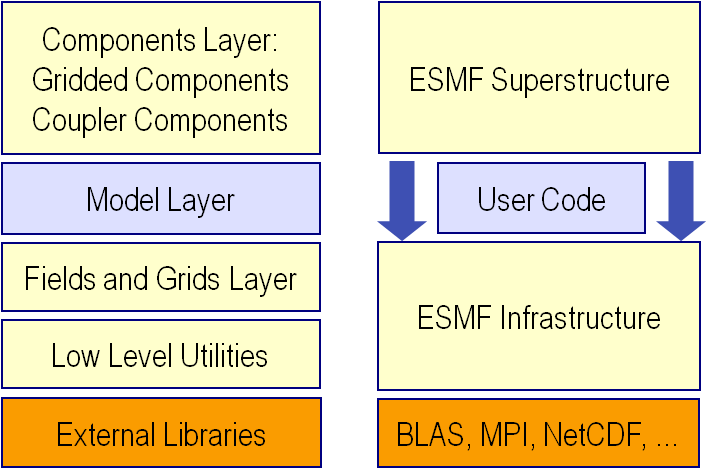
\includegraphics[width=0.6\textwidth]{pics/esmf/Figure1.png}
\caption{Schematic of the ESMF (sandwich) architecture}
\label{fig:Schematic of the ESMF (sandwich) architecture}
\end{figure}

The ESMF architecture is scalable, flexible paradigm for building highly complex climate, weather, and related applications from components such as land models, atmospheric models, and data assimilation systems. The ESMF is a way of developing components which can be used in many different user written applications. Model components that adopt ESMF can be used in different contexts with minimal code modification. Furthermore they may be incorporated into other ESMF-based modeling systems within the Earth science community. The components can create and drive other components. In order to take the outputs from one component and transform them into the inputs that are needed to run another component, couplers is used. In ESMF, couplers are also software components.

\emph{Superstructure layer}\\
The ESMF superstructure is a unifying context. User components are interconnected with this context. The superstructure is the means by which models are converted into components and coupled.\\
Classes called Gridded Components, Coupler Components, and States are used within the superstructure to achieve this flexibility. Gridded Components are major Earth system model components such as land surface models, ocean models, atmospheric models and sea ice models. Components used for linear algebra manipulations for example in state estimation are also created as Gridded Components.\\

The Figure \ref{fig:Building block for an ESMF application} shows a typical building block for an ESMF application consists of 
a parent Gridded Component, several child Gridded Components, and a Coupler Component. The parent Gridded Component is called by an application driver. All ESMF Components have initialize, run, and finalize methods. The diagram shows that when the application driver calls initialize on a parent Gridded Component, the call cascades down to all of its children. The result is that the entire (tree) of Components is initialized. The run and finalize methods work on the same principle. In this example a hurricane simulation is built from atmosphere and ocean Gridded Components. An atmosphere-ocean Coupler Component handles the data exchange between the ocean and atmosphere.

\begin{figure}[htbp]
\centering
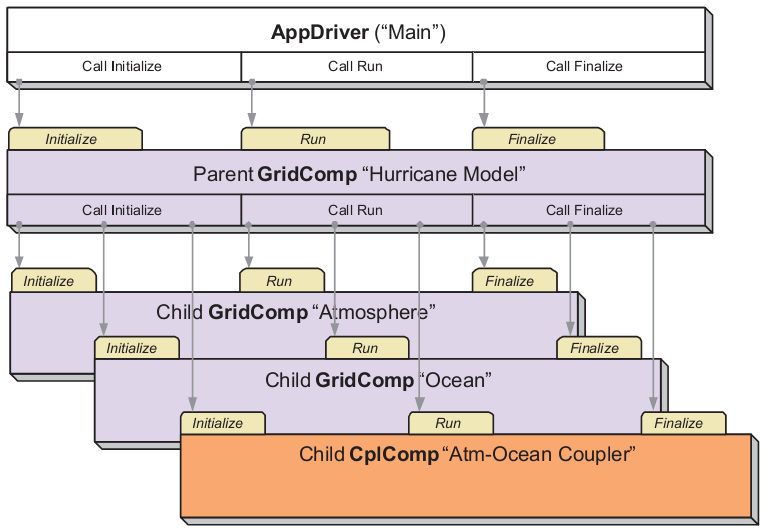
\includegraphics[width=0.6\textwidth]{pics/esmf/Figure2.png}
\caption{Building block for an ESMF application}
\label{fig:Building block for an ESMF application}
\end{figure}

User code components under ESMF use special interface objects for Component to Component data exchanges. These objects are of type import State and export State. The methods of these types allows user code components to do things like fill an export State object with data to be shared with other components or query an import State object to determine its contents.\\
The import State and export State abstractions are designed to be flexible enough so that ESMF does not need to mandate a single format for fields. For example, ESMF does not prescribe the units of quantities exported or imported. However, ESMF does provide mechanisms to describe units, memory layout, and grid coordinates. This allows the ESMF software to support a range of different policies for physical fields.\\
The Gridded Component class describes a user component that takes in one import State and produces one export State, shown in Figure \ref{fig:Architecture-Components and States}.

\begin{figure}[htbp]
\centering
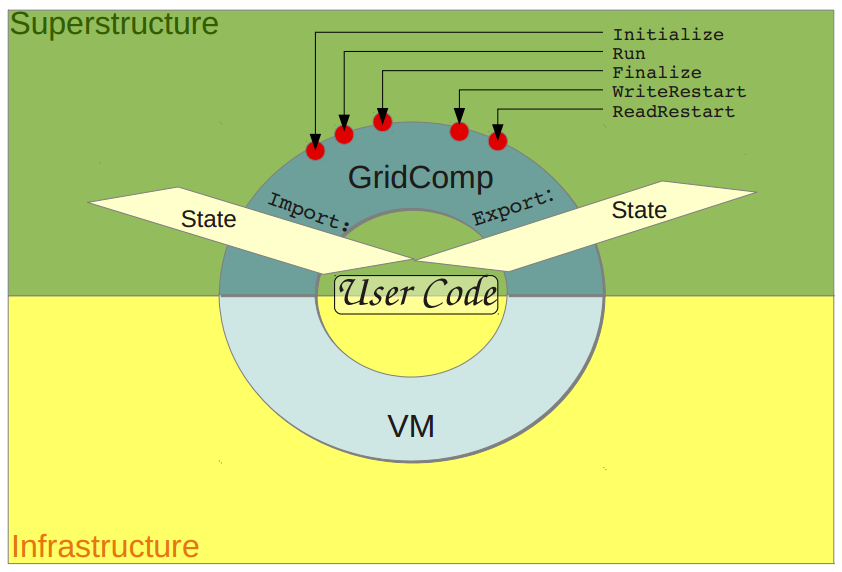
\includegraphics[width=0.6\textwidth]{pics/esmf/Figure3.png}
\caption{Architecture-Components and States}
\label{fig:Architecture-Components and States}
\end{figure}

\emph{Infrastructure layer}\\
Infrastructure is a standard software platform for enabling interoperability (developing couplers, ensuring performance portability). The infrastructure layer represents support for Physical Grids, Regridding, Decomposition/composition, Communication, Calendar and Time, I/O, Logging and Profiling. The infrastructure represents data structures and tools (Utilities) that modelers can use within their own code.\\

\emph{Data structures}\\
Model data is contained in a hierarchy of data structures. The user can reference a Fortran array to an ESMF Array or Field, or retrieve a Fortran array out of an ESMF Array or Field.\\

\begin{itemize}
	\item Array: holds a Fortran array (with other info, such as halo size)
	\item Field: holds an ESMF Array, an associated Grid, and metadata
	\item Bundle: collection of Fields on the same Grid bundled together for convenience and data locality. Bundles are intended for performance optimization, by sharing collective communication, IO, and regridding
\end{itemize}

\emph{Utilities}\\
\begin{itemize}
	\item Time Manager Utilities include Calendar, Clock (needed for superstructure), Time, Time interval, Alarm. These can be used independently of other ESMF utilities.
	\item Configuration Attributes (replaces namelists)
	\item Message logging (methods for writing error, warning \& informational messages)
\end{itemize}

\emph{Integration of user model in ESMF}\\
The steps for converting a user model into an ESMF component are mentioned here:\\
\begin{enumerate}
\item Separate code into a new module with initialize, run, and finalize stages
\item Create register routine
\begin{itemize}
	\item Register the initialize, run, and finalize routines
	\item Make the register routine public
\end{itemize}
\item Include framework module
\end{enumerate}

\emph{Hello World App}\\
Hello World App in Fortran. For ESMF, Hello World demonstrates a single component driven from one layer above using SetServices() and Gridded Components in practice, shown in Figure \ref{fig:Hello World App in Fortran}.

\begin{figure}[htbp]
\centering
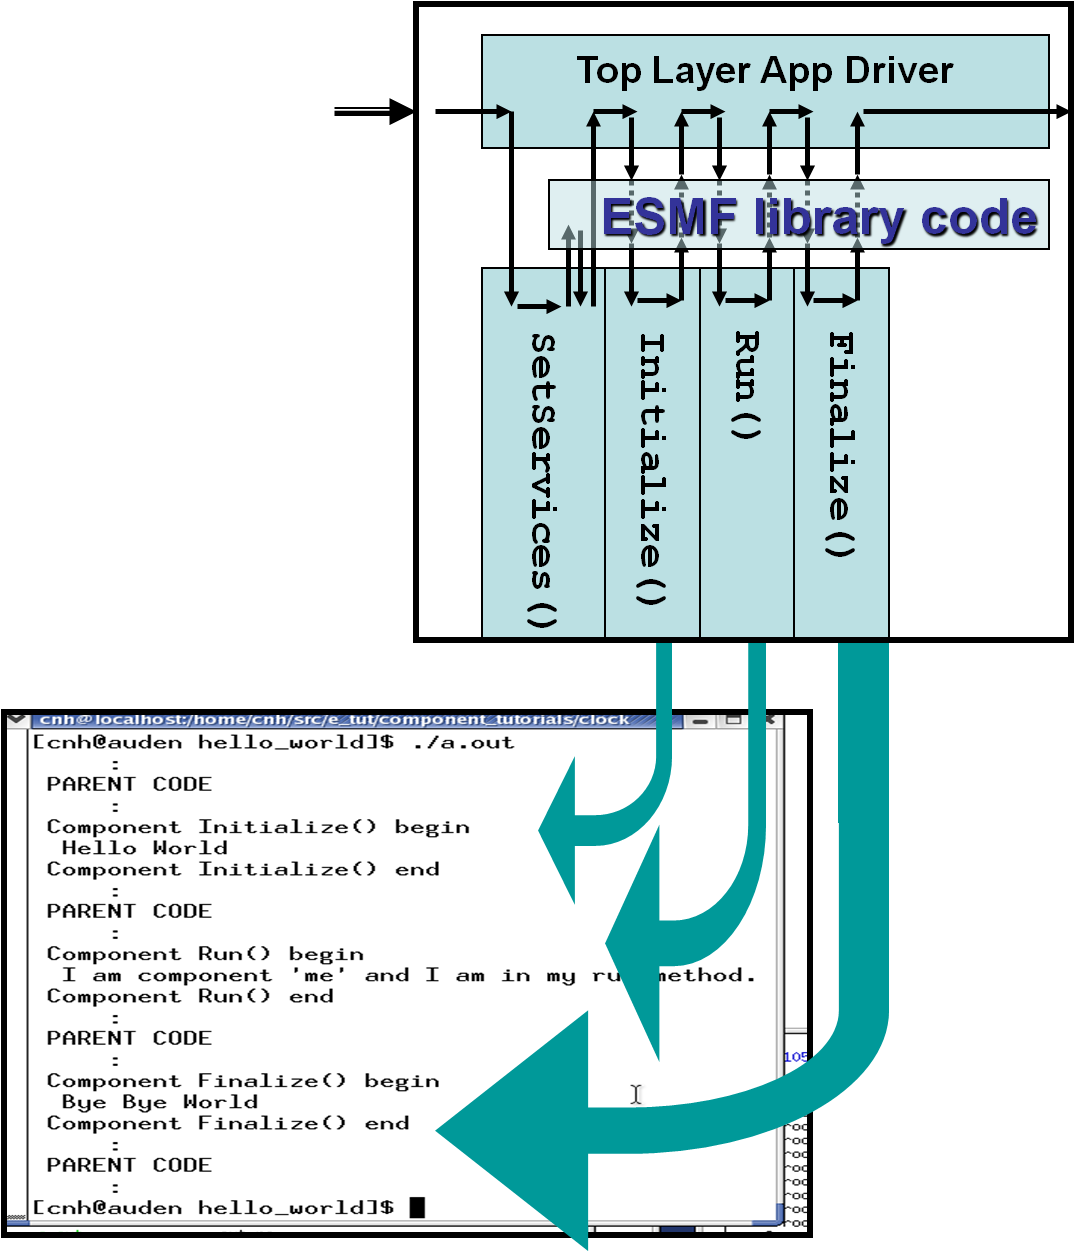
\includegraphics[width=0.6\textwidth]{pics/esmf/Figure4.png}
\caption{Hello World App in Fortran}
\label{fig:Hello World App in Fortran}
\end{figure}

Hello World in Fortran has two source files:\\
\begin{itemize}
	\item MyWorldGridCompMod.F90 contains the SetServices(), Initialize(), Run() and Finalize() code.
	\item hello\_world\_app.F90 contains the top layer app driver.
\end{itemize}


\emph{Properties of the modeling}\\
In ESMF, user data are represented in the form of data objects such as grids, fields, and arrays. The user data within a component may be copied or referenced into these ESMF objects. ESMF can associate metadata with data objects. The metadata, in the form of name and value pairs, is grouped into packages. These metadata packages can be written out in XML and other standard formats.\\

\subsubsection{Object-based modeling:}
The ESMF Application Programming Interface (API) is based on the object-oriented programming concept of a class.
\subsubsection{Flexible data and control flow:}
Import States, export States, Gridded Components and Coupler Components can be arrayed flexibly within a superstructure layer. Using these constructs, it is possible to configure a set of concurrently executing Gridded Components joined through a single Coupler Component of the style shown in Figure \ref{fig:ESMF supports configurations with a single central Coupler Component}. It is also possible to configure a set of Components with multiple point to point Coupler Components shown in Figure \ref{fig:ESMF configurations with multiple point to point Coupler Components}.  The set of superstructure abstractions allows flexible data flow and control between components. However, components will often use different discrete grids, and time-stepping components may march forward with different time intervals. The ESMF infrastructure layer provides elements to manage this complexity.

\begin{figure}[htbp]
\centering
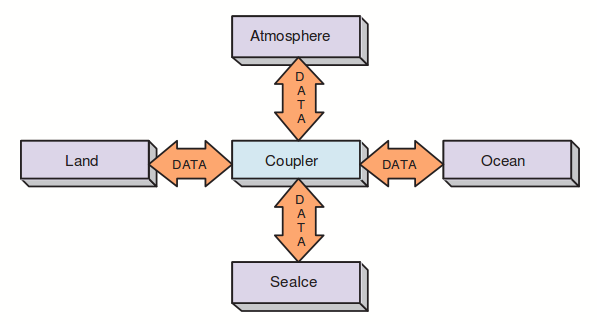
\includegraphics[width=0.6\textwidth]{pics/esmf/Figure5.png}
\caption{ESMF supports configurations with a single central Coupler Component}
\label{fig:ESMF supports configurations with a single central Coupler Component}
\end{figure}

\begin{figure}[htbp]
\centering
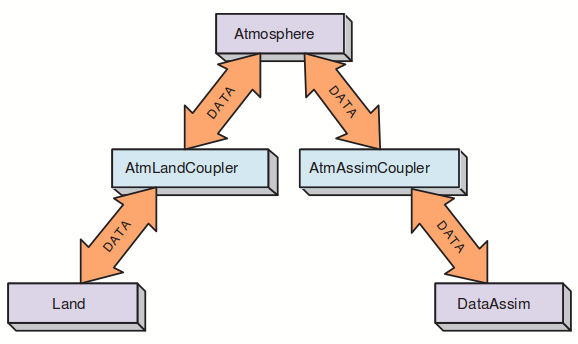
\includegraphics[width=0.6\textwidth]{pics/esmf/Figure6.png}
\caption{ESMF configurations with multiple point to point Coupler Components}
\label{fig:ESMF configurations with multiple point to point Coupler Components}
\end{figure}

\subsubsection{Parallel computing:}
ESMF runs on most high performance parallel computing platforms, including IBM, many Linux variants, Cray, Compaq, more. It supports Message Passing Interface (MPI), Open Multi-Processing (OpenMP) and hybrid user codes.
\subsubsection{Sequential execution:}
ESMF supports sequential mode (Single Program Multiple Datastream) but only very limited concurrent mode (Multiple Program Multiple Datastream) of execution.
\subsubsection{System Dynamics:}
The major classes in the ESMF superstructure are Components, which typically represent large pieces of functionality such as models, model couplers, dynamics and physics packages, and States, which are the data structures used to communicate data between Components.
\subsubsection{Visual modeling:}
ESMF provides regridding, also called remapping or interpolation. Regridding may be needed when communicating data between Earth system model components such as land and atmosphere, or between different data sets to support operations such as visualization.
\subsubsection{Modular modeling:}
ESMF is a software package for building modular, high performance modeling and data assimilation applications.\\

\emph{Pros and Cons}\\
ESMF provides a toolkit that components use to increase interoperability, improve performance portability and reuse common utility code. Componentization is simplified by dividing user models into initialize, finalize, and run routines. The process is scalable, because additional components are created the same way.\\
The framework provides a set of portable, robust, performance optimized libraries for data transfers, time management, and other common modeling functions. In order to take advantage of the ESMF infrastructure users should extensively rewrite their codes. Or users may decide to wrap user-written components in ESMF interfaces in order to adopt the ESMF architecture and use framework coupling services.\\

\subsubsection{Single execution mode:}
It is not expected that a single Gridded Component be able to function in both sequential and concurrent modes, although Gridded Components of different types can be nested. For example, a concurrently called Gridded Component can contain several nested sequential Gridded Components.
\subsubsection{No Transforms:}
Components must exchange data through ESMF-State objects. The input data are available at the time the user Component code is called, and data to be returned to another Component are available when that code returns.\\

In a coupled ocean-atmosphere model, for example, the task of replacing one ocean model with another model from a different organization often requires a major redevelopment effort. One of the main goals of the ESMF is to develop a standard interface which will clearly separate model component and couplers, so that interoperable components can be shared and reused.


\subsection{OMS (Object Modeling System)}
OMS stands for Object Modeling System designed for environmental modeling. It is a collaborative project carried out by US Department of Agriculture and other partner organizations, which are involved in agro-environmental modeling. The OMS is a component-based software framework for environmental model development, data provisioning, testing, validation and deployment.\\
It allows the implementation of single or multiple process modules that can be developed or applied for custom-tailored module configurations. With the help of the OMS framework, it is easier and more efficient for scientists to create or modify scientific models, simulate and run the models, analyze and evaluate the results. The OMS framework is an open source software system. Software developers can contribute to the OMS framework by adding new features to the existing framework to improve the performance of the framework.\\

\emph{Technical Implementation}\\
The OMS framework consists of different software tools, which work together to form a modeling platform. Figure \ref{fig:Details of major OMS framework components} shows the architecture of the OMS framework

\begin{figure}[htbp]
\centering
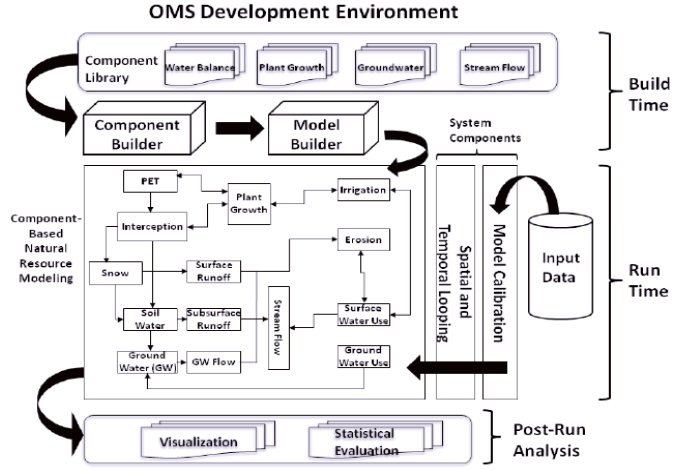
\includegraphics[width=0.6\textwidth]{pics/oms/Figure1.png}
\caption{Details of major OMS framework components}
\label{fig:Details of major OMS framework components}
\end{figure}

The architecture is made up of different layers, each of which has their own functions. In the top layer, there are component libraries, which provide the implementation of specific environmental processes, such as water balance, plant growth, and so on, to describe the behaviors of the environmental phenomena. The component builder utilizes the component libraries and supports the development of scientific components written in Java, FORTRAN, C or C++. The model builder provides the visual integration and configuration of complex models, which are composed of different standalone model components. It maps the output of one component to the input of subsequent components.\\
With the help of the component builder and model builder, multi-scientific components can be assembled to form a complex model. The OMS framework also provides simulation control over time and space, calibration tools for model analysis and control of data input and output. In the bottom layer, there are various tools for model data evaluation and visualization. The OMS framework provides tools to analyze the statistical data of model output and plot the result with different charts or diagrams for better understanding by the users.\\

\emph{Modeling Procedure of OMS}\\
OMS supports component based software engineering. Models and components are treated as objects in OMS. An individual component is a web service or a module that encapsulate a set of related functions separated from the surrounding framework environment.The OMS framework introduces a new approach of component modeling. In OMS framework, components are normal classes enriched with Java language level annotations. A normal class consists of fields and methods, which will be supplemented by language level annotations. The annotations are used to find the entry point of data flow and method execution. The computational method of a component will have a tag (@Execute) and data flows are indicated by the tags (@In) and (@Out).\\
The following example shows parts of a simple component of a bank account, whose financial credit varies year to year.\\

\begin{enumerate}
\item First we have to import the necessary annotation interfaces.
\begin{figure}[htbp]
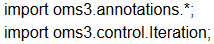
\includegraphics[width=0.3\textwidth]{pics/oms/Figure2.png}
\end{figure}

\item We can now use the annotations imported to indicate the data flow.
\begin{figure}[htbp]
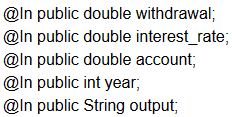
\includegraphics[width=0.3\textwidth]{pics/oms/Figure3.png}
\end{figure}


\item We can declare a computational function with the tag (@Execute), which processes the data flow.
\begin{figure}[htbp]
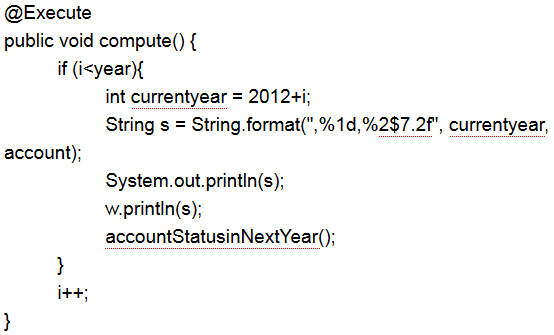
\includegraphics[width=0.6\textwidth]{pics/oms/Figure4.png}
\end{figure}

\item The annotation (@Finalize) indicates the framework that the following method will be executed at last to finalize the processing of data flow.
\begin{figure}[htbp]
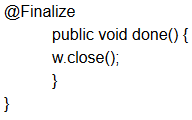
\includegraphics[width=0.3\textwidth]{pics/oms/Figure5.png}
\end{figure}
\end{enumerate}

The OMS framework provides simulations features to test and analyze the models, since it makes use of the advantages domain specific language, which are provided by the Groovy programming language. An OMS simulation provides all the necessary resources to run a model and it consists of following parts:
\begin{itemize}
	\item model and component executables, the core component to run and to be tested
	\item model specific parameter to indicate the input and output of data flow
	\item some strategies for handling output
	\item evaluate the model result with statistics or visualization
\end{itemize}

The following is a part of a simple simulation file to run the model (bank account).
\begin{enumerate}
\item We have to import the necessary library
\begin{figure}[htbp]
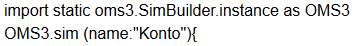
\includegraphics[width=0.5\textwidth]{pics/oms/Figure6.png}
\end{figure}

\item define the location of the components
\begin{figure}[htbp]
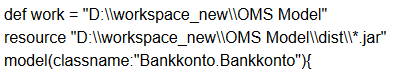
\includegraphics[width=0.5\textwidth]{pics/oms/Figure7.png}
\end{figure}

\item specify the input data for the components
\begin{figure}[htbp]
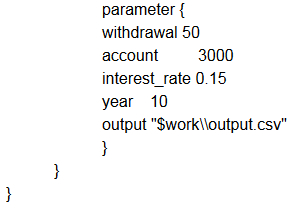
\includegraphics[width=0.4\textwidth]{pics/oms/Figure8.png}
\end{figure}
\end{enumerate}

The following figure shows the result after running the simulation.
\begin{figure}[htbp]
\centering
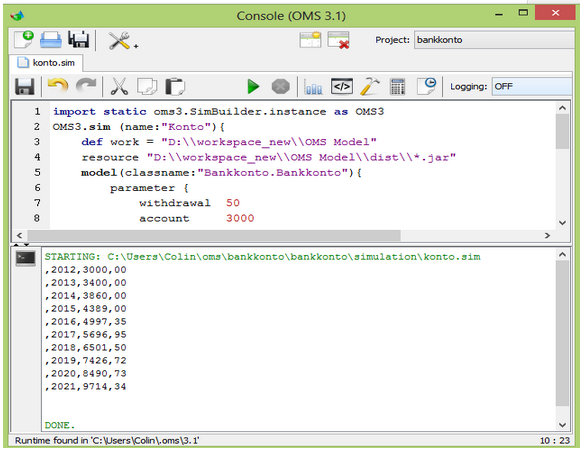
\includegraphics[width=0.6\textwidth]{pics/oms/Figure9.png}
\caption{Result after running the model (bank account)}
\label{fig:Result after running the model (bank account)}
\end{figure}

OMS also provides diagram visualization features for the simulation results for better understanding and evaluation. The following figure shows the diagram of the status changes of the bank account of different years.
\begin{figure}[htbp]
\centering
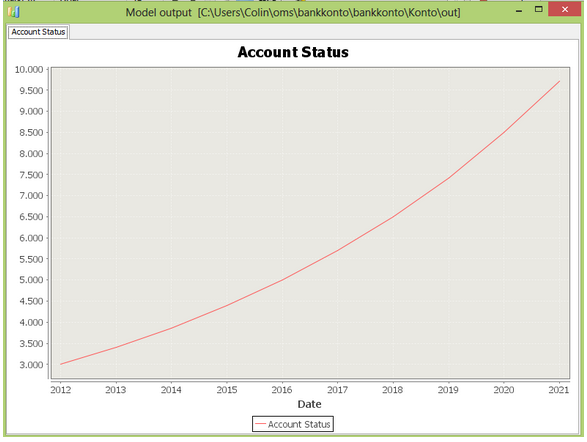
\includegraphics[width=0.6\textwidth]{pics/oms/Figure10.png}
\caption{Visualization of the status of a bank account}
\label{fig:Visualization of the status of a bank account}
\end{figure}

The new version of the OMS framework 3.1 supports multiple threading. Each OMS3 component will be executed in a separate thread, which is managed by the framework runtime. Thread communication happens when data flow from the (@Out) field of one component to the (@In) field of another component is carried out. The component will wait until all its necessary inputs are present and satisfied, then it starts to execute. Since modern computers are equipped with multi-core processors, the multi-threading feature will greatly make use of the power of the processors to improve the performance of the framework.

\emph{Modeling Procedure of OMS}\\
The OMS framework provides the following benefits for model developers:
\begin{enumerate}
\item The OMS framework enables efficient transfer of technology. The OMS framework provides a multi-dimensional platform for integration of various software tools, therefore, it is efficient to transfer of natural resource technology tools to other researchers or users. Due to the common modeling platform and common user interface, the OMS will reduce the start-up time of model development and lower training costs of users.

\item The OMS framework reduces the costs of developing new software technologies. In the past, the development of software components requires huge amount of investment and many scientists. With OMS, model developers can put scientific knowledge into packages as modules in OMS to build new customized software packages at a small fraction of costs.

\item Model developers are able to apply the most suitable science to a specific problem. The OMS provides various software tools, so that model developers can select the most appropriate modules available depending on the concrete natural problems and situations.

\item The OMS framework allows model developers to analyze the natural resource system production efficiently. The OMS provides an integration of software tools for effective analysis of natural resource system production and conservation issues, such as environmental quality, global climate change management, etc.

\item The OMS framework enhances productivity of researchers and scientists. With OMS, model developers can create customized, best-quality software tools. Field scientists will benefit from this advantage, because they can transfer the result directly to other soil and climate. Model developers now focus on the science module implementation, other than graphical user interface, deployment, etc, which helps to increase the productivity and quality. 
\end{enumerate}

\emph{Disadvantages of OMS}\\
Although the OMS framework provides various advantages for model developers, it also faces some difficulties.
\begin{enumerate}
\item Model developers always lack of motivation to share model code, for example, the component libraries of environmental processes, environmental models, etc. Therefore, model developers have to build their own modules repositories or contribute to the OMS module library, so that they are available for other model developers to do further developments. 
\item It is hard to predict whether a modular coding structure will be accepted or not. It will take much time for model developers to pay attention to the module design, especially the input and output requirements, module structure, meta data description, and proper use of annotations. In this way, the quality and usability of the module will be guaranteed.
\item Willingness to share data sets also affects the usability of the OMS framework. The data sets mentioned here are input or output of a model, for example, data for a range of natural resource processes covering different climatic and physio graphic regions across the world. Without these data sets, it is hard to reuse an existing model, since the data is important for comparison and evaluation. Without proper comparison and evaluation, further development of the existing model is almost impossible.
\end{enumerate}


\section{problems}
\section{declarative modelling}
\section{semantic approaches}